\chapter{Ohm's Law}

\section{Aim}
To find out how current varies with potential difference across an ohmic conductor

\section{Background Information}
When a voltage is applied across a conductor in any closed circuit, current flows through it. The amount of current that flows depends on the potential difference and the properties of the conductor.

The relationship between voltage and current is important for domestic purposes in cooking, charging mobile phones, producing light, radio, television and other industrial activities. Therefore there is a need to find out how the current varies with potential difference.


\section{Materials}
Voltmeter (0-3 V), Ammeter (0-3 A), Unknown Ohmic Resistor, 2 dry cells each 1.5 V size D, Switch and connecting wires

\section{Procedure}
\begin{enumerate}
\item Connect battery $E$, Ammeter $A$, Rheostat $Rh$, Ohmic Resistor $R$ and Switch $K$ in series (see figure).
\item Connect the voltmeter across (in parallel with) $R$.
\item Adjust the slide on the rheostat so that it is closest to $R$. This should give the maximum deflection of the Ammeter.
\item Record the values of current $I$ and potential difference $V$ in tabular form.
\item Obtain four more readings of $V$ and $I$ by moving the slider away from $R$ on the rheostat.
\end{enumerate}

\begin{figure}[h!]
\centering
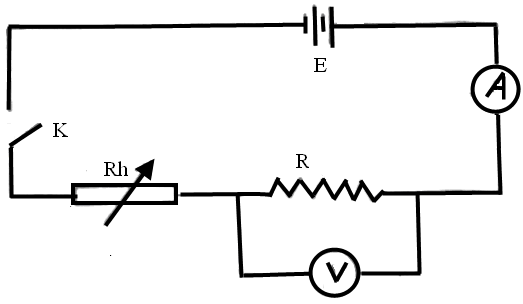
\includegraphics[width=10cm]{./img/ohms-law-1.png}
\caption{Ohm's Law practical setup}
\label{fig:ohms-law-1}
\end{figure}

\section{Analysis and Interpretation}
\begin{enumerate}
\item Draw the graph of $V$ against $I$.
\item From the graph; calculate the slope ($G$). What does this slope represent?
\item What do you think the $y$-intercept of the graph represents?
\item Consider an ohmic conductor with voltage of 6 V across it and resistor with a current of 2 A going through it. What is the resistance of the conductor?
\end{enumerate}

\section{Conclusion}
Explain how the current varies with potential difference in an ohmic conductor from the experiment.

\section{Questions for Discussion}
\begin{enumerate}
\item Suppose you plot the graph of $I$ against $V$, what would be the nature of the graph?
\item Why might it be important to have a constant temperature environment when conducting this experiment?
\item What are the sources of error in this experiment and how do they affect your results?
\end{enumerate}

\section{Reflection and Self Assessment}
\begin{enumerate}
\item Do you understand everything in this experiment? If not, explain what and in what ways can you improve your understanding?
\item Why is the information of this experiment important for circuit construction?
\end{enumerate}